\chapter{Endereçamento} \label{net_project}

\section{Atribuição de endereços} \label{ip_list}

De acordo com a estrutura da rede e as suas dependências, foi elaborado o seguinte endereçamento da rede:

\begin{table}[H]
    \begin{center}
        \begin{tabular}{ | c | c | c | c | c |}
        \hline
        \textbf{Endereço IP} & \textbf{Network} & \textbf{Broadcast} & \textbf{DNS} & \textbf{Gateway} \\ 
        \hline
        \textbf{Sede} & 192.168.0.0/23 & 192.168.1.255 & - & 192.168.1.254\\ 
        \hline
        \textbf{Rede de Servidores} & 192.168.2.224/29 & 192.168.2.231 & 192.168.2.225 & 192.168.2.230\\ 
        \hline
        \textbf{Armazém} & 192.168.2.192/27 & 192.168.2.223 & 192.168.2.193 & 192.168.2.222\\ 
        \hline
        \textbf{Loja1 - Vlan1} & 192.168.2.0/27 & 192.168.2.31 & 192.168.2.1 & 192.168.2.30\\ 
        \hline
        \textbf{Loja1 - Vlan2} & 192.168.2.32/27 & 192.168.2.63 & 192.168.2.33 & 192.168.2.62\\ 
        \hline
        \textbf{Loja2 - Vlan1} & 192.168.2.64/27 & 192.168.2.95 & 192.168.2.65 & 192.168.2.94\\ 
        \hline
        \textbf{Loja2 - Vlan2} & 192.168.2.96/27 & 192.168.2.127 & 192.168.2.97 & 192.168.2.126\\ 
        \hline
        \textbf{Loja3 - Vlan1} & 192.168.2.128/27 & 192.168.2.159 & 192.168.2.129 & 192.168.2.158\\ 
        \hline
        \textbf{Loja3 - Vlan2} & 192.168.2.160/27 & 192.168.2.191 & 192.168.2.161 & 192.168.2.190\\ 
        \hline
        \textbf{DMZ} & 20.49.51.160/28 & 20.49.51.175 & 20.49.51.161 & 20.49.51.174\\ 
        \hline
        \end{tabular}
    \end{center}
    \caption{Endereços dos elementos da rede}
    \label{tab:ip_table}
\end{table}

\section{Configuração na bancada} \label{bench_conf}

Para simular a tipologia da rede empresarial, foi criada a seguinte estrutura de rede na bancada:

\begin{table}[H]
    \begin{center}
        \begin{tabular}{ | c | c | c | }
        \hline
        \textbf{Host} & \textbf{Eth1} & \textbf{Eth2}\\ 
        \hline
        \textbf{Tux12} & Desativada & DNS Cache Armazém\\ 
        \hline
        \textbf{Tux13} & DNS Rede de Servidores & DNS DMZ\\ 
        \hline
        \textbf{Tux14} & DNS Loja 1 - Vlan1 & DNS Loja 1 - Vlan2\\ 
        \hline
        \end{tabular}
    \end{center}
    \caption{Estrutura de rede nos hosts}
    \label{tab:tux_table}
\end{table}

Para se obter esta tipologia, as respetivas interfaces foram configuradas deste modo:

\begin{figure}[H]
    \centering
    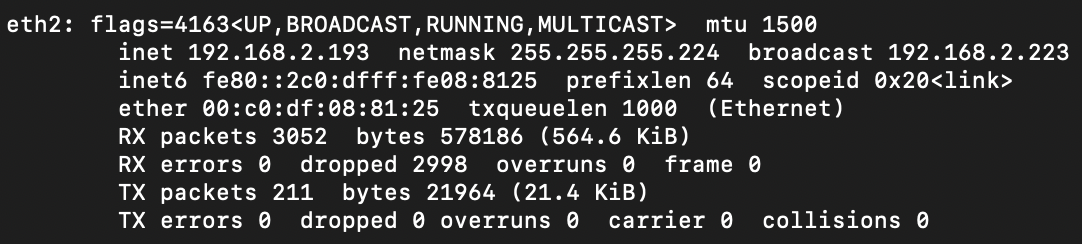
\includegraphics[width=.8\linewidth]{figs/tux_interfaces/tux12.png}
    \caption{Tux12 Interfaces}
    \label{fig:tux12}
\end{figure}

\begin{figure}[H]
    \centering
    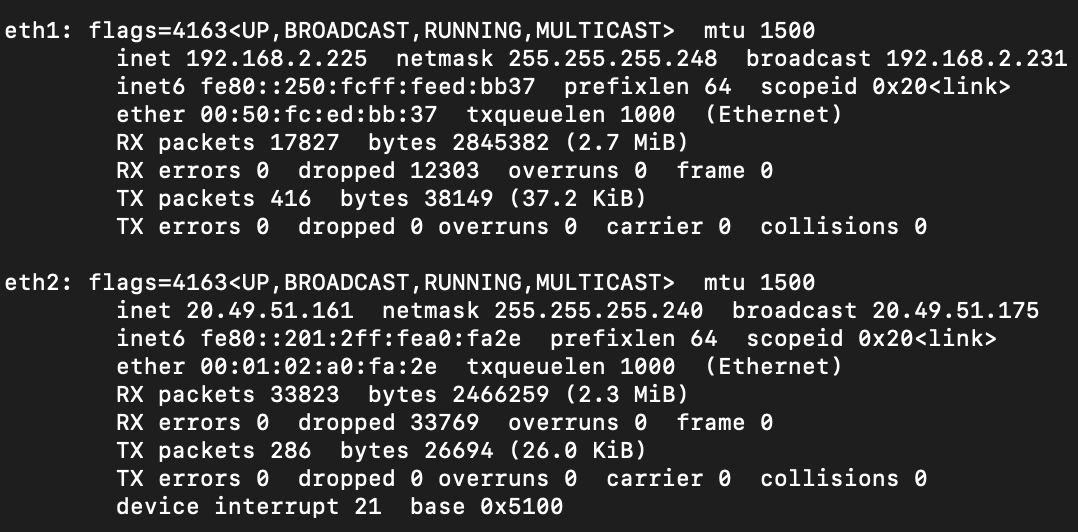
\includegraphics[width=.8\linewidth]{figs/tux_interfaces/tux13.png}
    \caption{Tux13 Interfaces}
    \label{fig:tux13}
\end{figure}

\begin{figure}[H]
    \centering
    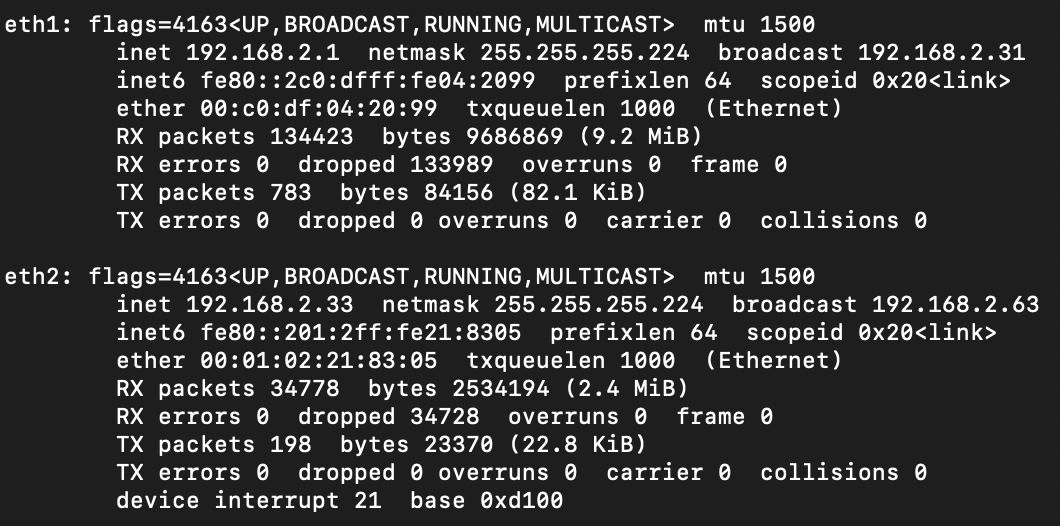
\includegraphics[width=.8\linewidth]{figs/tux_interfaces/tux14.png}
    \caption{Tux14 Interfaces}
    \label{fig:tux14}
\end{figure}

\section{Switch / Router} \label{switch_router}

A estrutura de rede apresentada requere que os diferentes sistemas estejam em Vlans diferentes, de forma a que o seu tráfego interno seja separado.
Para tal, várias Vlans foram configuradas no Switch de bancada, atribuindo as portas a que as interfaces dos Tux's estavam ligadas às Vlans respetivas \cite{vlan}:

\begin{figure}[H]
    \centering
    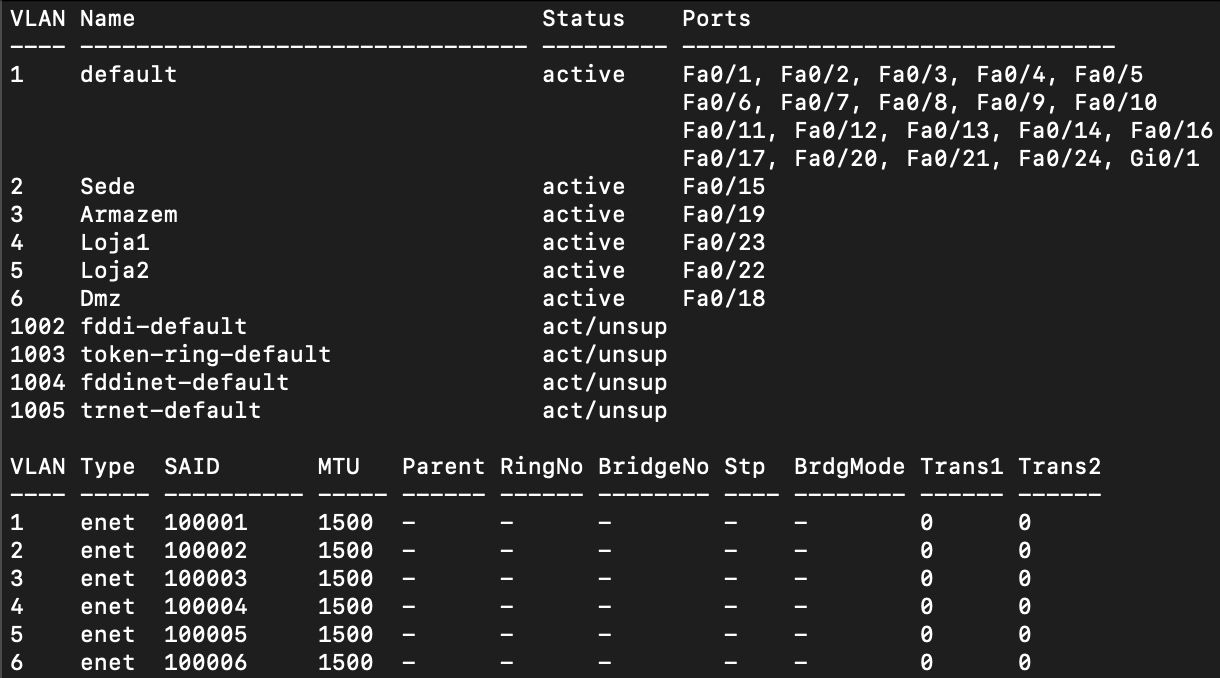
\includegraphics[width=.8\linewidth]{figs/roas/switch_vlans.png}
    \caption{Switch Vlans}
    \label{fig:switch_vlans}
\end{figure}

O switch não faz \textit{forward} de pacotes entre diferentes Vlans.
Desse modo, se queremos que as vlans possam comunicar entre si, temos que fazer uso de um dispositivo que suporte \textit{routing }Layer 3.
Neste caso, esse dispositivo é router de bancada, o que nos obriga a usar a abordagem \textbf{ROAS} (Router-on-a-stick).

Apenas existe uma interface que liga o Switch ao Router : GigabitEthernet2.
A configuração ROAS permite que esta interface seja dividida em sub-interfaces, cada uma delas associada a uma VLAN \cite{encapsulation}.
Estas sub-interfaces vão funcionar como as Gateways das diferentes Vlans no router.

O primeiro passo é criar um \textbf{Trunk} no Switch na interface que liga ao Router, que junte todas as vlans.
Esta trunk permite que as vlans sejam discriminadas à chegada ao router através do encapsulamento \textit{dot1Q}.

\begin{figure}[H]
    \centering
    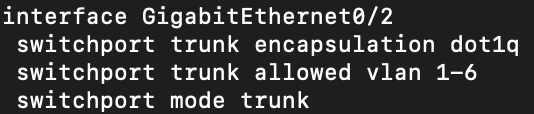
\includegraphics[width=.6\linewidth]{figs/roas/switch_trunk.png}
    \caption{Switch Trunk}
    \label{fig:switch_trunk}
\end{figure}

\clearpage

Após a criação do trunk, conseguimos no router separar as Vlans que estão nesse trunk e atribuir a cada uma a sua Gateway.

\begin{figure}[H]
    \centering
    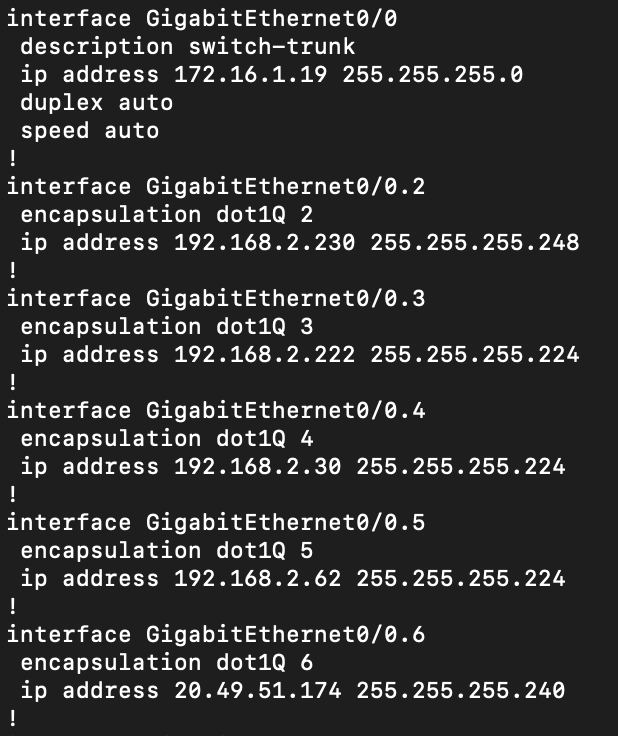
\includegraphics[width=.7\linewidth]{figs/roas/router.png}
    \caption{Router Interfaces}
    \label{fig:router_interfaces}
\end{figure}

Ao configurar o router, atribuímos a cada Vlan a sua \textit{Gateway}, assim como a sua \textit{Netmask} correspondente.
Deste modo, virtualizamos uma ligação direta individual de cada Vlan ao router.

Para testar a configuração podemos fazer um \textit{traceroute} entre duas Vlans distintas:

\begin{figure}[H]
    \centering
    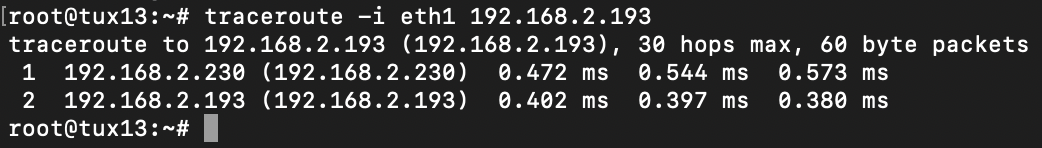
\includegraphics[width=.7\linewidth]{figs/roas/traceroute.png}
    \caption{Traceroute da Rede servidores para o Armazém}
    \label{fig:traceroute}
\end{figure}

Podemos observar que a Vlan da rede de servidores faz uso da sua gateway para aceder ao DNS da Vlan do Armazém.